\begin{figure}[!htbp]\centering
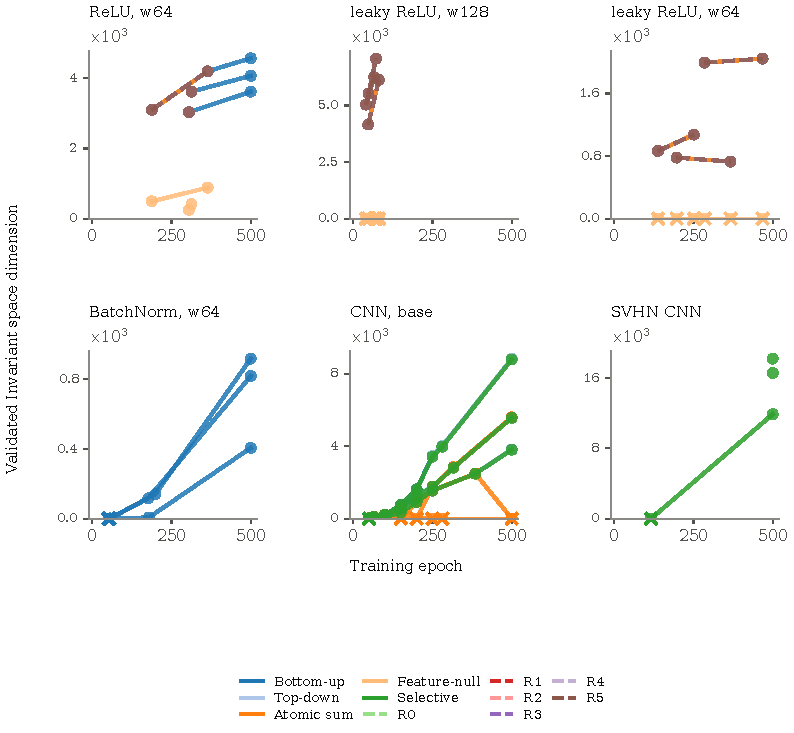
\includegraphics[width=4.762in]{construction_time_general_00.pdf}
\caption{Multilayer invariant subspace dimensions versus actual checkpoint epoch. Each curve is one seed; colors identify constructions, and dashed curves denote random layer orders R0--R5. Coincident curves have equal retained dimensions. Crosses mark zero retained dimension, including failed validations; unattempted constructions have no point. MNIST is used unless labeled SVHN. Only models with a trajectory measured within at least one seed are shown.}
\end{figure}
\FloatBarrier
